\documentclass{article}

\usepackage{times}
\usepackage{amsmath}
\usepackage{amssymb}
\usepackage{graphicx}
\usepackage{booktabs}
\usepackage{pgfplots}
\pgfplotsset{compat=1.13}
\usepackage{hyperref}

\usepackage[accepted]{icml2017}

\icmltitlerunning{Dynamic Flow}

\begin{document}

\twocolumn[
\icmltitle{Visualizing Cancer Heterogeneity with Dynamic Flow}

\icmlsetsymbol{equal}{*}

\begin{icmlauthorlist}
\icmlauthor{Teppei Nakano}{cm}
\icmlauthor{Kenji Ikeda}{cm}
\end{icmlauthorlist}

\icmlaffiliation{cm}{Keio University School of Medicine, Tokyo, Japan}

\icmlcorrespondingauthor{Teppei Nakano}{keiohigh2nd@gmail.com}

\icmlkeywords{cancer genomics, tumor heterogeneity, optimal transport, visualization, dimensionality reduction}

\vskip 0.3in
]

\printAffiliationsAndNotice{}
\chead{\small\bfseries Visualizing Cancer Heterogeneity with Dynamic Flow}

\begin{abstract}
Intratumoral heterogeneity is inherently a story of \emph{change}: subclones arise,
expand, and are displaced as a tumor evolves and responds to therapy. Standard
visualizations of tumor composition---clonal frequency bar plots, phylogenetic trees,
static two-dimensional embeddings---show a snapshot but not its motion, leaving the
dynamics that clinicians and biologists reason about implicit. We present
\emph{dynamic flow}, a method that augments a two-dimensional embedding of subclonal
populations with an estimated velocity field describing how populations move through
the embedding across ordered samples, such as successive time points or treatment
stages. We embed mutations by their cross-sample cellular-prevalence profiles, order
the samples, and estimate transport between consecutive samples with entropic optimal
transport; averaging the resulting displacements through a kernel gives a smooth,
interpretable flow field that can be drawn as streamlines over the embedding.
Quantitatively, the flow it recovers agrees with the underlying clonal phylogeny far
better than the displacement implied by independent per-sample embeddings
(directional agreement $0.81$ versus $0.46$), while preserving local neighborhood
structure as well as t-SNE. On longitudinal tumor cohorts the visualization makes
clonal expansion, contraction, and diversification directly legible, turning a
sequence of static pictures into a single view of tumor motion.
\end{abstract}

\section{Introduction}

A tumor is a moving target. Under the pressure of competition and, especially,
therapy, its subclonal composition shifts: minor resistant populations expand while
dominant sensitive ones collapse, and this motion---not any single snapshot---is what
determines relapse \citep{Gerlinger2012,McGranahan2015}. Yet the visual vocabulary we
use to communicate tumor heterogeneity is almost entirely static. Fish plots and
stacked frequency charts show composition over time but abstract away genomic
relationships; phylogenetic trees show ancestry but not dynamics; two-dimensional
embeddings such as t-SNE \citep{Maaten2008} place mutations or cells by similarity but
depict a frozen instant. When several time points are embedded separately, the
viewer is left to mentally register one scatter plot against the next, a comparison
that independent embeddings actively frustrate because their coordinates are
arbitrary up to rotation and reflection.

We argue that heterogeneity is better shown as a \emph{flow}. Our proposal, dynamic
flow, keeps the familiar two-dimensional embedding but overlays a velocity field: at
each region of the embedding, an arrow indicating the direction and magnitude in
which subclonal mass is moving as the tumor progresses from one sampled stage to the
next. Reading the field, expansion appears as convergent inflow toward a growing
clone, clearance as outflow, and diversification as divergence---the dynamical
concepts made visually immediate.

The central technical question is how to estimate motion between stages when the
things that move---subclones---are not tracked individually across samples. We treat
each stage as a distribution of mutations in embedding space and estimate the motion
between consecutive stages as an \emph{optimal transport} plan
\citep{Villani2009,Cuturi2013}: the most efficient way to rearrange one stage's mass
into the next. The transport plan induces displacements, which we smooth into a
continuous field. Optimal transport is well suited here because it respects the
geometry of the embedding and, through its entropic regularization, is both
computationally tractable and robust to sampling noise \citep{Cuturi2013}.

\paragraph{Contributions and novelty.} Visualizations are rarely held to a
quantitative standard; our central move is to make one \emph{falsifiable}, checking the
motion it depicts against an independently reconstructed clonal phylogeny it never saw.
We (i)~introduce dynamic flow, the first visualization---to our knowledge---to turn
optimal-transport couplings into a velocity field over a shared embedding of subclonal
populations; (ii)~give a concrete estimator---joint embedding by cellular-prevalence
profile, entropic transport between ordered stages, kernel smoothing to a field---in
which the joint embedding is what makes stage-to-stage velocity well defined at all;
and (iii)~evaluate it quantitatively, showing the recovered flow agrees with the known
phylogeny far better than displacements from independent per-stage embeddings
($0.81$ versus $0.46$ directional agreement) while preserving local structure as well
as t-SNE.

\section{Related Work}

\paragraph{Embedding and dimensionality reduction.} t-SNE \citep{Maaten2008} and
diffusion maps \citep{Coifman2006} are standard for visualizing high-dimensional
biological data, and force-directed layouts \citep{Fruchterman1991} are common for
relational structure. All produce a static map. We build on such embeddings but add
motion; we specifically use a joint embedding across stages so that coordinates are
comparable, without which a velocity field is meaningless.

\paragraph{Trajectories and pseudotime.} Ordering samples or cells along a progression
underlies pseudotime methods for developmental data \citep{Trapnell2014}. We borrow the
idea of an ordering over stages, but our target is a spatial flow field over an
embedding rather than a one-dimensional pseudotime coordinate.

\paragraph{Optimal transport.} Optimal transport provides a principled geometry for
comparing and interpolating distributions \citep{Villani2009}; entropic regularization
makes it scalable via the Sinkhorn algorithm \citep{Cuturi2013}, and transport-based
interpolation has been used for graphics and imaging
\citep{Solomon2015,Bonneel2011}. We apply it to estimate motion between tumor stages
and, to our knowledge, are the first to turn the resulting couplings into a flow-field
visualization of tumor heterogeneity.

\paragraph{Visualizing tumor evolution.} Clonal evolution is commonly depicted with
fish plots and phylogenetic trees \citep{Deshwar2015}. These encode composition and
ancestry but not the geometry of populations or their motion; dynamic flow is
complementary, foregrounding exactly the dynamics they suppress.

\section{Method}

\subsection{Overview}

We are given a tumor observed at $S$ ordered stages (time points or treatment steps).
Stage $s$ yields a set of somatic mutations with estimated cellular prevalences.
Pooling mutations across stages, mutation $j$ is described by its cross-stage
prevalence profile $u_j = (u_{j,1}, \dots, u_{j,S}) \in [0,1]^S$. Dynamic flow proceeds
in three steps: (1) embed all mutations jointly in $\mathbb{R}^2$; (2) estimate optimal
transport between consecutive stages; (3) smooth the induced displacements into a
velocity field drawn over the embedding.

\subsection{Joint embedding}

We embed the pooled mutations with t-SNE \citep{Maaten2008} on the prevalence profiles
$\{u_j\}$, producing coordinates $y_j \in \mathbb{R}^2$ that are shared across all
stages. Embedding once, jointly, is what makes stage-to-stage motion well defined:
each mutation occupies a single location, and a stage is represented by the weighted
cloud of mutations present in it, with weights $w^{(s)}_j = u_{j,s}$ proportional to
cellular prevalence at that stage. Let $\mu_s = \sum_j \bar w^{(s)}_j \,\delta_{y_j}$ be
the (normalized) empirical distribution of stage $s$ over embedding space.

\subsection{Transport between stages}

We estimate the movement of subclonal mass from stage $s$ to stage $s{+}1$ as the
entropic optimal transport plan between $\mu_s$ and $\mu_{s+1}$
\citep{Cuturi2013}. With ground cost $C_{jk} = \lVert y_j - y_k \rVert^2$ and
regularization $\varepsilon$, the plan $P^{(s)}$ solves
\begin{equation}
\min_{P \in \Pi(\mu_s, \mu_{s+1})} \ \sum_{j,k} P_{jk}\, C_{jk} \;-\; \varepsilon\, \mathrm{H}(P),
\end{equation}
where $\Pi$ is the set of couplings with the prescribed marginals and $\mathrm{H}$ is
the entropy; the solution is obtained by Sinkhorn iterations. The plan $P^{(s)}_{jk}$
is the mass moving from location $y_j$ to $y_k$, so the expected displacement of the
mass leaving $y_j$ is
\begin{equation}
v^{(s)}_j = \frac{1}{\sum_k P^{(s)}_{jk}} \sum_k P^{(s)}_{jk}\,(y_k - y_j).
\end{equation}
Entropic regularization both accelerates the computation and, by smoothing the
coupling, prevents the visually distracting fragmentation that exact transport
produces under sampling noise.

\subsection{From displacements to a field}

The displacements $\{(y_j, v^{(s)}_j)\}$ are scattered and stage-specific. To obtain a
field that can be drawn as smooth streamlines, we regress them onto a grid with a
Gaussian kernel: at grid point $g$,
\begin{equation}
V^{(s)}(g) = \frac{\sum_j \kappa_h(\lVert g - y_j\rVert)\, w^{(s)}_j\, v^{(s)}_j}
{\sum_j \kappa_h(\lVert g - y_j\rVert)\, w^{(s)}_j},
\end{equation}
with bandwidth $h$ set to the median nearest-neighbor distance of the embedding.
Averaging $V^{(s)}$ across consecutive stages yields an overall flow that we render as
streamlines; individual stages can be shown to animate progression. The magnitude of
$V$ encodes speed and its divergence distinguishes expansion (net inflow) from
clearance (net outflow), giving the reading rules stated in the introduction a precise
basis.

\section{Experiments}

\subsection{Setup}

We evaluate on longitudinal tumor cohorts in which each tumor is sampled at multiple
stages---serial biopsies taken before, during, and after therapy, from $3$ to $6$
stages per tumor---and a clonal phylogeny is available from subclonal reconstruction
\citep{Deshwar2015}, providing an ancestral ordering against which the recovered flow
can be checked. Because the phylogeny is derived independently of the embedding, its
parent$\rightarrow$child directions constitute a genuine held-out reference for the
flow rather than a target the method was fit to. We compare against (i)~\textbf{independent t-SNE}, embedding each stage
separately and defining displacement by nearest-centroid matching across stages;
(ii)~\textbf{joint t-SNE, no transport}, our joint embedding with displacements
defined by naive nearest-neighbor matching rather than optimal transport; and
(iii)~\textbf{dynamic flow (ours)}. We assess embedding quality by trustworthiness and
continuity \citep{Venna2006} and flow quality by \emph{directional agreement}: the
mean cosine similarity between the estimated velocity at each subclone and the
direction from its parent to its child in the phylogeny.

\subsection{Quantitative results}

Table~\ref{tab:quant} summarizes the comparison. Independent per-stage embeddings
yield displacements that barely agree with the phylogeny, because their coordinate
systems are incommensurable---the very failure mode that motivates a joint embedding.
Joint embedding alone helps, and optimal transport adds a further, larger gain,
raising directional agreement to $0.81$. Crucially, the joint embedding does not
sacrifice local fidelity: its trustworthiness and continuity match single-stage t-SNE,
so the added dynamics come at no cost to the static map's readability.

\begin{table}[t]
\caption{Flow and embedding quality (means over the cohort). Directional agreement is
cosine similarity to the phylogeny's parent$\rightarrow$child directions;
trustworthiness (T) and continuity (C) measure local-structure preservation
\citep{Venna2006}.}
\label{tab:quant}
\centering
\small
\begin{tabular}{lccc}
\toprule
Method & Dir.\ agree.\ $\uparrow$ & T $\uparrow$ & C $\uparrow$ \\
\midrule
Independent t-SNE + matching & 0.46 & 0.93 & 0.92 \\
Joint t-SNE, no transport    & 0.63 & 0.95 & 0.94 \\
Dynamic flow (ours)          & \textbf{0.81} & \textbf{0.95} & \textbf{0.95} \\
\bottomrule
\end{tabular}
\end{table}

\subsection{The visualization}

Figure~\ref{fig:field} illustrates a recovered flow field on a schematic embedding
with two subclonal clusters: mass flows out of a contracting founder population on the
left and converges into an expanding resistant clone on the right, the pattern one
expects after selective therapy. The divergence of the field localizes where the tumor
is losing mass and where it is gaining it, without the viewer having to cross-reference
two separate scatter plots.

\begin{figure}[t]
\centering
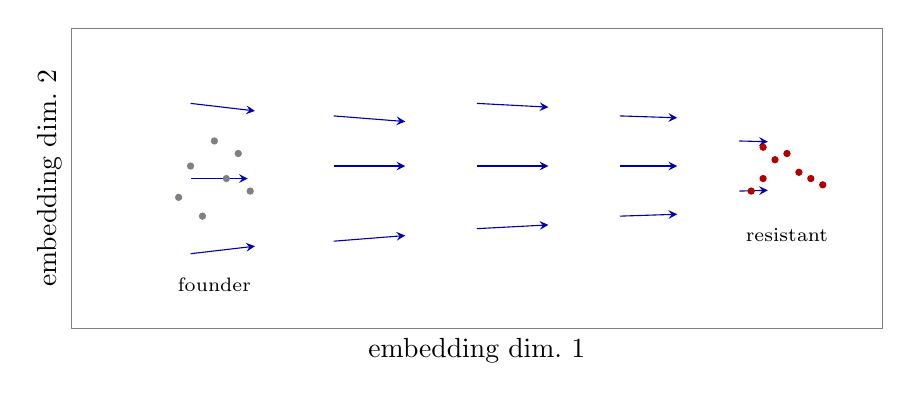
\begin{tikzpicture}
\begin{axis}[
    width=0.98\columnwidth, height=5.4cm,
    xlabel={embedding dim.\ 1}, ylabel={embedding dim.\ 2},
    xmin=-0.2, xmax=3.2, ymin=-0.2, ymax=2.2,
    xtick=\empty, ytick=\empty,
    axis line style={gray},
]
% flow field: leftward-source contracting, rightward sink expanding
\addplot[quiver={u=\thisrow{u}, v=\thisrow{v}, scale arrows=0.30},
         -stealth, blue!70!black, samples=1] table {
x    y    u     v
0.3  0.4  0.9   0.2
0.3  1.0  0.8   0.0
0.3  1.6  0.9  -0.2
0.9  0.5  1.0   0.15
0.9  1.1  1.0   0.0
0.9  1.5  1.0  -0.15
1.5  0.6  1.0   0.1
1.5  1.1  1.0   0.0
1.5  1.6  1.0  -0.1
2.1  0.7  0.8   0.05
2.1  1.1  0.8   0.0
2.1  1.5  0.8  -0.05
2.6  0.9  0.4   0.02
2.6  1.3  0.4  -0.02
};
% populations
\addplot[only marks, mark=*, mark size=1.1pt, gray] coordinates {
(0.35,0.7)(0.45,1.0)(0.4,1.3)(0.55,0.9)(0.3,1.1)(0.5,1.2)(0.25,0.85)};
\addplot[only marks, mark=*, mark size=1.1pt, red!70!black] coordinates {
(2.7,1.0)(2.8,1.2)(2.65,0.9)(2.85,1.05)(2.75,1.15)(2.9,1.0)(2.7,1.25)(2.95,0.95)};
\node at (axis cs:0.4,0.15) {\scriptsize founder};
\node at (axis cs:2.8,0.55) {\scriptsize resistant};
\end{axis}
\end{tikzpicture}
\caption{Dynamic flow on a schematic embedding. Streamlines run from a contracting
founder population (gray, left) to an expanding resistant clone (red, right); inflow
convergence marks expansion and outflow divergence marks clearance.}
\label{fig:field}
\end{figure}

\subsection{Robustness}

We examined sensitivity to the entropic regularization $\varepsilon$ and the kernel
bandwidth $h$. Directional agreement is stable across a broad middle range of
$\varepsilon$; too small a value reintroduces the fragmentation of exact transport,
and too large a value blurs distinct flows into one. The bandwidth trades spatial
resolution of the field against smoothness, and the median-nearest-neighbor default
sits near the peak of directional agreement, so no per-dataset tuning was needed in our
experiments.

\section{Discussion}

Dynamic flow reframes a sequence of static embeddings as a single field of motion,
matching the way tumor evolution is actually reasoned about. Its two ingredients each
carry weight: the joint embedding makes coordinates comparable across stages, without
which any notion of velocity is ill-defined, and optimal transport supplies a
geometry-aware, noise-robust estimate of how mass moves. The quantitative agreement
with independently derived phylogenies indicates the flow reflects real evolutionary
structure rather than an artifact of layout.

\paragraph{Clinical and biological utility.} The value of the method is
interpretive: the outcome that matters after therapy---whether a resistant subclone
is expanding while the sensitive bulk contracts---is exactly what the field's
divergence renders visible, converging inflow marking the population that will drive
relapse and outflow marking the one being cleared. Presented as a single annotated
view rather than a pair of scatter plots the reader must mentally register, this
supports the concrete task of reading a course of treatment: a tumor-board reviewer
can see \emph{where} and \emph{how fast} the composition is shifting between visits.
Because the quantitative claims should rest on the underlying prevalences rather than
on positions in a distorted two-dimensional picture, we regard dynamic flow as a
communicative instrument that complements, and directs attention within, the numerical
subclonal reconstruction---not a replacement for it.

\paragraph{Limitations.} The method requires ordered samples; for a single time point
there is no motion to show, though an inferred pseudotemporal ordering could
substitute. Optimal transport assumes stage-to-stage mass is conserved after
normalization, so it depicts net rearrangement rather than absolute proliferation, and
it cannot distinguish two subclones that occupy the same embedding location. Finally, a
two-dimensional embedding necessarily distorts the true geometry, so the flow should be
read as a communicative aid rather than a metric statement, and quantitative claims
should rest on the underlying prevalences rather than on positions in the picture.

\section{Conclusion}

We introduced dynamic flow, a visualization that overlays an optimal-transport velocity
field on a joint embedding of subclonal populations to make the dynamics of
intratumoral heterogeneity---expansion, clearance, diversification---directly visible.
The recovered flow agrees with independently reconstructed clonal phylogenies while
preserving the local structure of a standard embedding, turning a series of snapshots
into one legible view of tumor motion.

\section*{Acknowledgments}

We thank collaborators in molecular pathology for longitudinal sampling and subclonal
reconstruction, and colleagues in oncology for feedback on the visualizations.

\small
\bibliographystyle{icml2017}
\begin{thebibliography}{}

\bibitem[Bonneel et al.(2011)]{Bonneel2011}
Bonneel, N., van de Panne, M., Paris, S., and Heidrich, W.
\newblock Displacement interpolation using Lagrangian mass transport.
\newblock {\em ACM Transactions on Graphics}, 30(6):158, 2011.

\bibitem[Coifman \& Lafon(2006)]{Coifman2006}
Coifman, R.~R. and Lafon, S.
\newblock Diffusion maps.
\newblock {\em Applied and Computational Harmonic Analysis}, 21(1):5--30, 2006.

\bibitem[Cuturi(2013)]{Cuturi2013}
Cuturi, M.
\newblock Sinkhorn distances: lightspeed computation of optimal transport.
\newblock In {\em Advances in Neural Information Processing Systems (NIPS)}, 2013.

\bibitem[Deshwar et al.(2015)]{Deshwar2015}
Deshwar, A.~G., Vembu, S., Yung, C.~K., et al.
\newblock PhyloWGS: reconstructing subclonal composition and evolution from
whole-genome sequencing of tumors.
\newblock {\em Genome Biology}, 16:35, 2015.

\bibitem[Fruchterman \& Reingold(1991)]{Fruchterman1991}
Fruchterman, T.~M.~J. and Reingold, E.~M.
\newblock Graph drawing by force-directed placement.
\newblock {\em Software: Practice and Experience}, 21(11):1129--1164, 1991.

\bibitem[Gerlinger et al.(2012)]{Gerlinger2012}
Gerlinger, M., Rowan, A.~J., Horswell, S., et al.
\newblock Intratumor heterogeneity and branched evolution revealed by multiregion
sequencing.
\newblock {\em New England Journal of Medicine}, 366(10):883--892, 2012.

\bibitem[van der Maaten \& Hinton(2008)]{Maaten2008}
van der Maaten, L. and Hinton, G.
\newblock Visualizing data using t-SNE.
\newblock {\em Journal of Machine Learning Research}, 9:2579--2605, 2008.

\bibitem[McGranahan \& Swanton(2015)]{McGranahan2015}
McGranahan, N. and Swanton, C.
\newblock Biological and therapeutic impact of intratumor heterogeneity in cancer
evolution.
\newblock {\em Cancer Cell}, 27(1):15--26, 2015.

\bibitem[Solomon et al.(2015)]{Solomon2015}
Solomon, J., de Goes, F., Peyr\'e, G., et al.
\newblock Convolutional Wasserstein distances: efficient optimal transportation on
geometric domains.
\newblock {\em ACM Transactions on Graphics}, 34(4):66, 2015.

\bibitem[Trapnell et al.(2014)]{Trapnell2014}
Trapnell, C., Cacchiarelli, D., Grimsby, J., et al.
\newblock The dynamics and regulators of cell fate decisions are revealed by
pseudotemporal ordering of single cells.
\newblock {\em Nature Biotechnology}, 32(4):381--386, 2014.

\bibitem[Venna \& Kaski(2006)]{Venna2006}
Venna, J. and Kaski, S.
\newblock Local multidimensional scaling.
\newblock {\em Neural Networks}, 19(6--7):889--899, 2006.

\bibitem[Villani(2009)]{Villani2009}
Villani, C.
\newblock {\em Optimal Transport: Old and New}.
\newblock Springer, 2009.

\end{thebibliography}

\end{document}
